\documentclass[twoside]{book}

% Packages required by doxygen
\usepackage{fixltx2e}
\usepackage{calc}
\usepackage{doxygen}
\usepackage[export]{adjustbox} % also loads graphicx
\usepackage{graphicx}
\usepackage[utf8]{inputenc}
\usepackage{makeidx}
\usepackage{multicol}
\usepackage{multirow}
\PassOptionsToPackage{warn}{textcomp}
\usepackage{textcomp}
\usepackage[nointegrals]{wasysym}
\usepackage[table]{xcolor}

% Font selection
\usepackage[T1]{fontenc}
\usepackage[scaled=.90]{helvet}
\usepackage{courier}
\usepackage{amssymb}
\usepackage{sectsty}
\renewcommand{\familydefault}{\sfdefault}
\allsectionsfont{%
  \fontseries{bc}\selectfont%
  \color{darkgray}%
}
\renewcommand{\DoxyLabelFont}{%
  \fontseries{bc}\selectfont%
  \color{darkgray}%
}
\newcommand{\+}{\discretionary{\mbox{\scriptsize$\hookleftarrow$}}{}{}}

% Page & text layout
\usepackage{geometry}
\geometry{%
  a4paper,%
  top=2.5cm,%
  bottom=2.5cm,%
  left=2.5cm,%
  right=2.5cm%
}
\tolerance=750
\hfuzz=15pt
\hbadness=750
\setlength{\emergencystretch}{15pt}
\setlength{\parindent}{0cm}
\setlength{\parskip}{3ex plus 2ex minus 2ex}
\makeatletter
\renewcommand{\paragraph}{%
  \@startsection{paragraph}{4}{0ex}{-1.0ex}{1.0ex}{%
    \normalfont\normalsize\bfseries\SS@parafont%
  }%
}
\renewcommand{\subparagraph}{%
  \@startsection{subparagraph}{5}{0ex}{-1.0ex}{1.0ex}{%
    \normalfont\normalsize\bfseries\SS@subparafont%
  }%
}
\makeatother

% Headers & footers
\usepackage{fancyhdr}
\pagestyle{fancyplain}
\fancyhead[LE]{\fancyplain{}{\bfseries\thepage}}
\fancyhead[CE]{\fancyplain{}{}}
\fancyhead[RE]{\fancyplain{}{\bfseries\leftmark}}
\fancyhead[LO]{\fancyplain{}{\bfseries\rightmark}}
\fancyhead[CO]{\fancyplain{}{}}
\fancyhead[RO]{\fancyplain{}{\bfseries\thepage}}
\fancyfoot[LE]{\fancyplain{}{}}
\fancyfoot[CE]{\fancyplain{}{}}
\fancyfoot[RE]{\fancyplain{}{\bfseries\scriptsize Generated by Doxygen }}
\fancyfoot[LO]{\fancyplain{}{\bfseries\scriptsize Generated by Doxygen }}
\fancyfoot[CO]{\fancyplain{}{}}
\fancyfoot[RO]{\fancyplain{}{}}
\renewcommand{\footrulewidth}{0.4pt}
\renewcommand{\chaptermark}[1]{%
  \markboth{#1}{}%
}
\renewcommand{\sectionmark}[1]{%
  \markright{\thesection\ #1}%
}

% Indices & bibliography
\usepackage{natbib}
\usepackage[titles]{tocloft}
\setcounter{tocdepth}{3}
\setcounter{secnumdepth}{5}
\makeindex

% Hyperlinks (required, but should be loaded last)
\usepackage{ifpdf}
\ifpdf
  \usepackage[pdftex,pagebackref=true]{hyperref}
\else
  \usepackage[ps2pdf,pagebackref=true]{hyperref}
\fi
\hypersetup{%
  colorlinks=true,%
  linkcolor=blue,%
  citecolor=blue,%
  unicode%
}

% Custom commands
\newcommand{\clearemptydoublepage}{%
  \newpage{\pagestyle{empty}\cleardoublepage}%
}

\usepackage{caption}
\captionsetup{labelsep=space,justification=centering,font={bf},singlelinecheck=off,skip=4pt,position=top}

%===== C O N T E N T S =====

\begin{document}

% Titlepage & ToC
\hypersetup{pageanchor=false,
             bookmarksnumbered=true,
             pdfencoding=unicode
            }
\pagenumbering{alph}
\begin{titlepage}
\vspace*{7cm}
\begin{center}%
{\Large ppl-\/\+Assignment-\/\+I\+I\+T2015071 \\[1ex]\large v2.\+0 }\\
\vspace*{1cm}
{\large Generated by Doxygen 1.8.13}\\
\end{center}
\end{titlepage}
\clearemptydoublepage
\pagenumbering{roman}
\tableofcontents
\clearemptydoublepage
\pagenumbering{arabic}
\hypersetup{pageanchor=true}

%--- Begin generated contents ---
\chapter{I\+P\+PL Assignment}
\label{md_readme}
\Hypertarget{md_readme}
\subsection*{Object Oriented Programming}

\subsubsection*{Piyush Arora -\/ I\+I\+T2015071}

\subsubsection*{Contents}


\begin{DoxyItemize}
\item \href{#build-details}{\tt Build Details}
\item \href{#testing-instructions}{\tt Testing Instructions}
\item \href{#documentation-and-class-diagrams}{\tt Documentation and Class Diagrams}
\item \href{#tools-used}{\tt Tools Used}
\end{DoxyItemize}

\subsection*{Build Details}

\subsubsection*{Language\+:}


\begin{DoxyCode}
C++
\end{DoxyCode}


\subsubsection*{Platform\+:}


\begin{DoxyCode}
VS Code Version 1.11.1
\end{DoxyCode}


\subsubsection*{Operating System\+:}


\begin{DoxyCode}
Windows 10 Insider Editor v1703 OS Build 15063.13
\end{DoxyCode}


\subsection*{Testing instructions}


\begin{DoxyItemize}
\item Generate random set (Boys, Girls, Gifts)\+: 
\begin{DoxyCode}
g++ GenerateBG.cpp && ./a.out
\end{DoxyCode}

\item Question 3\+: 
\begin{DoxyCode}
g++ Q03.cpp && ./a.out
\end{DoxyCode}

\item Question 4\+: 
\begin{DoxyCode}
g++ Q04.cpp && ./a.out
\end{DoxyCode}

\item Question 5\+: 
\begin{DoxyCode}
g++ Q05.cpp && ./a.out
\end{DoxyCode}
 $>$$\ast$$\ast$\+N\+O\+T\+E$\ast$$\ast$\+: For Q5, first run Generate\+BG since couples have to be reset;
\item Question 6\+: 
\begin{DoxyCode}
g++ Q06.cpp && ./a.out
\end{DoxyCode}

\item Question 7\+: 
\begin{DoxyCode}
g++ Q07.cpp && ./a.out
\end{DoxyCode}

\item Question 8\+: 
\begin{DoxyCode}
g++ Q08.cpp && ./a.out
\end{DoxyCode}
 $>$$\ast$$\ast$\+N\+O\+T\+E$\ast$$\ast$\+: For Q8, first run Generate\+BG since couples have to be reset and run Q03 first to make couples since if you run if after other questions and gifts may already be generated and have taken = 1, some data may be spoilt and may cause bugs. PS\+: just a precautionary step
\item All gift exchange events will be logged in {\ttfamily C\+S\+V/\+Gift\+Exchange\+Log.\+csv}
\item Utility functions are present in {\ttfamily Qx\+Utility.\+cpp (x = 3 to 8)}
\item .csv files are present in {\ttfamily C\+S\+V/}, and names used are present in {\ttfamily Names/}
\end{DoxyItemize}

\subsection*{Documentation and Class Diagrams}


\begin{DoxyItemize}
\item Documentation is available {\ttfamily documentation/}
\end{DoxyItemize}

\subsubsection*{Class Diagrams}


\begin{DoxyItemize}
\item All diagrams are already included in html documentation
\item Class diagram is separately present in {\ttfamily Class\+Diagram.\+png}
\end{DoxyItemize}

\subsection*{Tools Used}


\begin{DoxyItemize}
\item \href{http://www.stack.nl/~dimitri/doxygen/}{\tt doxygen} \+: Generates automatic documentation
\item \href{http://www.sparxsystems.com/products/ea/}{\tt Enterprise Architect} \+: Generates class diagram 
\end{DoxyItemize}
\chapter{Hierarchical Index}
\section{Class Hierarchy}
This inheritance list is sorted roughly, but not completely, alphabetically\+:\begin{DoxyCompactList}
\item \contentsline{section}{Couple}{\pageref{class_couple}}{}
\item \contentsline{section}{Gift}{\pageref{class_gift}}{}
\begin{DoxyCompactList}
\item \contentsline{section}{Essential\+Gift}{\pageref{class_essential_gift}}{}
\item \contentsline{section}{Luxury\+Gift}{\pageref{class_luxury_gift}}{}
\item \contentsline{section}{Utility\+Gift}{\pageref{class_utility_gift}}{}
\end{DoxyCompactList}
\item \contentsline{section}{Person}{\pageref{class_person}}{}
\begin{DoxyCompactList}
\item \contentsline{section}{Boy}{\pageref{class_boy}}{}
\item \contentsline{section}{Girl}{\pageref{class_girl}}{}
\end{DoxyCompactList}
\end{DoxyCompactList}

\chapter{Class Index}
\section{Class List}
Here are the classes, structs, unions and interfaces with brief descriptions\+:\begin{DoxyCompactList}
\item\contentsline{section}{\hyperlink{class_boy}{Boy} }{\pageref{class_boy}}{}
\item\contentsline{section}{\hyperlink{class_couple}{Couple} }{\pageref{class_couple}}{}
\item\contentsline{section}{\hyperlink{class_essential_gift}{Essential\+Gift} }{\pageref{class_essential_gift}}{}
\item\contentsline{section}{\hyperlink{class_gift}{Gift} }{\pageref{class_gift}}{}
\item\contentsline{section}{\hyperlink{class_girl}{Girl} }{\pageref{class_girl}}{}
\item\contentsline{section}{\hyperlink{class_luxury_gift}{Luxury\+Gift} }{\pageref{class_luxury_gift}}{}
\item\contentsline{section}{\hyperlink{class_person}{Person} }{\pageref{class_person}}{}
\item\contentsline{section}{\hyperlink{class_utility_gift}{Utility\+Gift} }{\pageref{class_utility_gift}}{}
\end{DoxyCompactList}

\chapter{Class Documentation}
\hypertarget{class_boy}{}\section{Boy Class Reference}
\label{class_boy}\index{Boy@{Boy}}
\subsection*{Public Member Functions}
\begin{DoxyCompactItemize}
\item 
\hyperlink{class_boy_a0a51d40be8680589d7ed43a64959fc8b}{Boy} (std\+::string name, int attractiveness, int budget, int intelligence\+Level, int type, int min\+Attraction)
\item 
std\+::string \hyperlink{class_boy_acf59fd0074a6ea3413751a95b2970303}{get\+Name} ()
\item 
int \hyperlink{class_boy_a814ef4919f2ac86c6ee70f9698afad3d}{get\+Attractiveness} ()
\item 
int \hyperlink{class_boy_a05c48b12091ebcad44ba86ba88514ac5}{get\+Budget} ()
\item 
\mbox{\Hypertarget{class_boy_a62c95b320fb02474cb339ddba96014d8}\label{class_boy_a62c95b320fb02474cb339ddba96014d8}} 
int {\bfseries get\+Intelligence\+Level} ()
\item 
bool \hyperlink{class_boy_a2aaabbf515640f59d44638b3ec7837b8}{is\+Committed} ()
\item 
std\+::string \hyperlink{class_boy_ae7faa071153b463f2a7424650b1f6db3}{get\+Partner} ()
\item 
int \hyperlink{class_boy_a65dcb5946aa7d736f15d7ca8d892dab7}{get\+Type} ()
\item 
double \hyperlink{class_boy_a7ab7e61631b30e7f679ba204f3b2616d}{get\+Happiness} ()
\item 
int \hyperlink{class_boy_a35d84533352a88f6365a28ba21b9f993}{get\+Min\+Attraction} ()
\item 
void \hyperlink{class_boy_a402b2082685030f1484f1c9940f4e977}{set\+Attractiveness} (int attractiveness)
\item 
void \hyperlink{class_boy_adb0aa7b4399c4d463129be2b2b9c3b42}{set\+Budget} (int budget)
\item 
void \hyperlink{class_boy_a6af3e7642f17781764a7aae58568d5c7}{set\+Committed} (bool committed)
\item 
void \hyperlink{class_boy_ad1eea5f50af9763a810bff01bb0a80e2}{set\+Intelligence\+Level} (int intelligence\+Level)
\item 
void \hyperlink{class_boy_a1762597ae2a5423ccb1583893b6622f6}{set\+Partner} (std\+::string partner)
\item 
void \hyperlink{class_boy_a7936f0d137ab929e118043a80067e43e}{set\+Type} (int type)
\item 
void \hyperlink{class_boy_a4de551a1a85cd44f8955ef3eea50eb0e}{set\+Happiness} (double happiness)
\item 
void \hyperlink{class_boy_a9e39b3cb4cbc2c0827a34410d9f826fc}{set\+Min\+Attraction} (int min\+Attraction)
\end{DoxyCompactItemize}


\subsection{Constructor \& Destructor Documentation}
\mbox{\Hypertarget{class_boy_a0a51d40be8680589d7ed43a64959fc8b}\label{class_boy_a0a51d40be8680589d7ed43a64959fc8b}} 
\index{Boy@{Boy}!Boy@{Boy}}
\index{Boy@{Boy}!Boy@{Boy}}
\subsubsection{\texorpdfstring{Boy()}{Boy()}}
{\footnotesize\ttfamily Boy\+::\+Boy (\begin{DoxyParamCaption}\item[{std\+::string}]{name,  }\item[{int}]{attractiveness,  }\item[{int}]{budget,  }\item[{int}]{intelligence\+Level,  }\item[{int}]{type,  }\item[{int}]{min\+Attraction }\end{DoxyParamCaption})}

Creates the boy 

\subsection{Member Function Documentation}
\mbox{\Hypertarget{class_boy_a814ef4919f2ac86c6ee70f9698afad3d}\label{class_boy_a814ef4919f2ac86c6ee70f9698afad3d}} 
\index{Boy@{Boy}!get\+Attractiveness@{get\+Attractiveness}}
\index{get\+Attractiveness@{get\+Attractiveness}!Boy@{Boy}}
\subsubsection{\texorpdfstring{get\+Attractiveness()}{getAttractiveness()}}
{\footnotesize\ttfamily int Boy\+::get\+Attractiveness (\begin{DoxyParamCaption}{ }\end{DoxyParamCaption})}

Returns boy\textquotesingle{}s attractiveness \mbox{\Hypertarget{class_boy_a05c48b12091ebcad44ba86ba88514ac5}\label{class_boy_a05c48b12091ebcad44ba86ba88514ac5}} 
\index{Boy@{Boy}!get\+Budget@{get\+Budget}}
\index{get\+Budget@{get\+Budget}!Boy@{Boy}}
\subsubsection{\texorpdfstring{get\+Budget()}{getBudget()}}
{\footnotesize\ttfamily int Boy\+::get\+Budget (\begin{DoxyParamCaption}{ }\end{DoxyParamCaption})}

Returns boy\textquotesingle{}s budget \mbox{\Hypertarget{class_boy_a7ab7e61631b30e7f679ba204f3b2616d}\label{class_boy_a7ab7e61631b30e7f679ba204f3b2616d}} 
\index{Boy@{Boy}!get\+Happiness@{get\+Happiness}}
\index{get\+Happiness@{get\+Happiness}!Boy@{Boy}}
\subsubsection{\texorpdfstring{get\+Happiness()}{getHappiness()}}
{\footnotesize\ttfamily double Boy\+::get\+Happiness (\begin{DoxyParamCaption}{ }\end{DoxyParamCaption})}

Returns happiness value \mbox{\Hypertarget{class_boy_a35d84533352a88f6365a28ba21b9f993}\label{class_boy_a35d84533352a88f6365a28ba21b9f993}} 
\index{Boy@{Boy}!get\+Min\+Attraction@{get\+Min\+Attraction}}
\index{get\+Min\+Attraction@{get\+Min\+Attraction}!Boy@{Boy}}
\subsubsection{\texorpdfstring{get\+Min\+Attraction()}{getMinAttraction()}}
{\footnotesize\ttfamily int Boy\+::get\+Min\+Attraction (\begin{DoxyParamCaption}{ }\end{DoxyParamCaption})}

Returns boy\textquotesingle{}s min attraction \mbox{\Hypertarget{class_boy_acf59fd0074a6ea3413751a95b2970303}\label{class_boy_acf59fd0074a6ea3413751a95b2970303}} 
\index{Boy@{Boy}!get\+Name@{get\+Name}}
\index{get\+Name@{get\+Name}!Boy@{Boy}}
\subsubsection{\texorpdfstring{get\+Name()}{getName()}}
{\footnotesize\ttfamily std\+::string Boy\+::get\+Name (\begin{DoxyParamCaption}{ }\end{DoxyParamCaption})}

Returns boy\textquotesingle{}s name \mbox{\Hypertarget{class_boy_ae7faa071153b463f2a7424650b1f6db3}\label{class_boy_ae7faa071153b463f2a7424650b1f6db3}} 
\index{Boy@{Boy}!get\+Partner@{get\+Partner}}
\index{get\+Partner@{get\+Partner}!Boy@{Boy}}
\subsubsection{\texorpdfstring{get\+Partner()}{getPartner()}}
{\footnotesize\ttfamily std\+::string Boy\+::get\+Partner (\begin{DoxyParamCaption}{ }\end{DoxyParamCaption})}

Returns partner \mbox{\Hypertarget{class_boy_a65dcb5946aa7d736f15d7ca8d892dab7}\label{class_boy_a65dcb5946aa7d736f15d7ca8d892dab7}} 
\index{Boy@{Boy}!get\+Type@{get\+Type}}
\index{get\+Type@{get\+Type}!Boy@{Boy}}
\subsubsection{\texorpdfstring{get\+Type()}{getType()}}
{\footnotesize\ttfamily int Boy\+::get\+Type (\begin{DoxyParamCaption}{ }\end{DoxyParamCaption})}

Returns type of boy \mbox{\Hypertarget{class_boy_a2aaabbf515640f59d44638b3ec7837b8}\label{class_boy_a2aaabbf515640f59d44638b3ec7837b8}} 
\index{Boy@{Boy}!is\+Committed@{is\+Committed}}
\index{is\+Committed@{is\+Committed}!Boy@{Boy}}
\subsubsection{\texorpdfstring{is\+Committed()}{isCommitted()}}
{\footnotesize\ttfamily bool Boy\+::is\+Committed (\begin{DoxyParamCaption}{ }\end{DoxyParamCaption})}

Returns commited status \mbox{\Hypertarget{class_boy_a402b2082685030f1484f1c9940f4e977}\label{class_boy_a402b2082685030f1484f1c9940f4e977}} 
\index{Boy@{Boy}!set\+Attractiveness@{set\+Attractiveness}}
\index{set\+Attractiveness@{set\+Attractiveness}!Boy@{Boy}}
\subsubsection{\texorpdfstring{set\+Attractiveness()}{setAttractiveness()}}
{\footnotesize\ttfamily void Boy\+::set\+Attractiveness (\begin{DoxyParamCaption}\item[{int}]{attractiveness }\end{DoxyParamCaption})}

Sets attractiveness \mbox{\Hypertarget{class_boy_adb0aa7b4399c4d463129be2b2b9c3b42}\label{class_boy_adb0aa7b4399c4d463129be2b2b9c3b42}} 
\index{Boy@{Boy}!set\+Budget@{set\+Budget}}
\index{set\+Budget@{set\+Budget}!Boy@{Boy}}
\subsubsection{\texorpdfstring{set\+Budget()}{setBudget()}}
{\footnotesize\ttfamily void Boy\+::set\+Budget (\begin{DoxyParamCaption}\item[{int}]{budget }\end{DoxyParamCaption})}

Sets budget \mbox{\Hypertarget{class_boy_a6af3e7642f17781764a7aae58568d5c7}\label{class_boy_a6af3e7642f17781764a7aae58568d5c7}} 
\index{Boy@{Boy}!set\+Committed@{set\+Committed}}
\index{set\+Committed@{set\+Committed}!Boy@{Boy}}
\subsubsection{\texorpdfstring{set\+Committed()}{setCommitted()}}
{\footnotesize\ttfamily void Boy\+::set\+Committed (\begin{DoxyParamCaption}\item[{bool}]{committed }\end{DoxyParamCaption})}

Sets commited status \mbox{\Hypertarget{class_boy_a4de551a1a85cd44f8955ef3eea50eb0e}\label{class_boy_a4de551a1a85cd44f8955ef3eea50eb0e}} 
\index{Boy@{Boy}!set\+Happiness@{set\+Happiness}}
\index{set\+Happiness@{set\+Happiness}!Boy@{Boy}}
\subsubsection{\texorpdfstring{set\+Happiness()}{setHappiness()}}
{\footnotesize\ttfamily void Boy\+::set\+Happiness (\begin{DoxyParamCaption}\item[{double}]{happiness }\end{DoxyParamCaption})}

Sets happiness \mbox{\Hypertarget{class_boy_ad1eea5f50af9763a810bff01bb0a80e2}\label{class_boy_ad1eea5f50af9763a810bff01bb0a80e2}} 
\index{Boy@{Boy}!set\+Intelligence\+Level@{set\+Intelligence\+Level}}
\index{set\+Intelligence\+Level@{set\+Intelligence\+Level}!Boy@{Boy}}
\subsubsection{\texorpdfstring{set\+Intelligence\+Level()}{setIntelligenceLevel()}}
{\footnotesize\ttfamily void Boy\+::set\+Intelligence\+Level (\begin{DoxyParamCaption}\item[{int}]{intelligence\+Level }\end{DoxyParamCaption})}

Sets intelligence level \mbox{\Hypertarget{class_boy_a9e39b3cb4cbc2c0827a34410d9f826fc}\label{class_boy_a9e39b3cb4cbc2c0827a34410d9f826fc}} 
\index{Boy@{Boy}!set\+Min\+Attraction@{set\+Min\+Attraction}}
\index{set\+Min\+Attraction@{set\+Min\+Attraction}!Boy@{Boy}}
\subsubsection{\texorpdfstring{set\+Min\+Attraction()}{setMinAttraction()}}
{\footnotesize\ttfamily void Boy\+::set\+Min\+Attraction (\begin{DoxyParamCaption}\item[{int}]{min\+Attraction }\end{DoxyParamCaption})}

Sets min attraction \mbox{\Hypertarget{class_boy_a1762597ae2a5423ccb1583893b6622f6}\label{class_boy_a1762597ae2a5423ccb1583893b6622f6}} 
\index{Boy@{Boy}!set\+Partner@{set\+Partner}}
\index{set\+Partner@{set\+Partner}!Boy@{Boy}}
\subsubsection{\texorpdfstring{set\+Partner()}{setPartner()}}
{\footnotesize\ttfamily void Boy\+::set\+Partner (\begin{DoxyParamCaption}\item[{std\+::string}]{partner }\end{DoxyParamCaption})}

Sets partner \mbox{\Hypertarget{class_boy_a7936f0d137ab929e118043a80067e43e}\label{class_boy_a7936f0d137ab929e118043a80067e43e}} 
\index{Boy@{Boy}!set\+Type@{set\+Type}}
\index{set\+Type@{set\+Type}!Boy@{Boy}}
\subsubsection{\texorpdfstring{set\+Type()}{setType()}}
{\footnotesize\ttfamily void Boy\+::set\+Type (\begin{DoxyParamCaption}\item[{int}]{type }\end{DoxyParamCaption})}

Sets type of boy

Type = 0 =$>$ Miser; Type = 1 =$>$ Generous; Type = 2 =$>$ Geeks; ! 

The documentation for this class was generated from the following files\+:\begin{DoxyCompactItemize}
\item 
C\+:/\+Users/\+Piyush Arora/\+Google Drive/\+Semester-\/4/\+Theory/\+I\+P\+P\+L430\+C/\+Assignment/Boy.\+h\item 
C\+:/\+Users/\+Piyush Arora/\+Google Drive/\+Semester-\/4/\+Theory/\+I\+P\+P\+L430\+C/\+Assignment/Boy.\+cpp\end{DoxyCompactItemize}

\hypertarget{class_couple}{}\section{Couple Class Reference}
\label{class_couple}\index{Couple@{Couple}}
\subsection*{Public Member Functions}
\begin{DoxyCompactItemize}
\item 
\hyperlink{class_couple_ade28403308aff7ddb1ac1e7ec7b94ebf}{Couple} (int index, int boy, int girl)
\item 
\hyperlink{class_couple_a6f82dc74dea2eac7998499841545a796}{Couple} (int index, int boy, int girl, double boy\+Happiness, double girl\+Happiness, double couple\+Happiness, double couple\+Compatibility, int total\+Money\+Spent, int total\+Value\+Gift, int total\+Lux\+Value)
\item 
int \hyperlink{class_couple_af83e7bba22f91af32166d757347c8331}{get\+Boy} ()
\item 
int \hyperlink{class_couple_a102761f3b3c46949a97829d518bfb0fe}{get\+Girl} ()
\item 
int \hyperlink{class_couple_adde1121effca72c7eb13f258c9caff47}{get\+Index} ()
\item 
\mbox{\Hypertarget{class_couple_a149c13daf2e50bcbaa2e8e11e2070972}\label{class_couple_a149c13daf2e50bcbaa2e8e11e2070972}} 
double {\bfseries get\+Boy\+Happiness} ()
\item 
\mbox{\Hypertarget{class_couple_a97b7e4b99943a7b00d64c7b2c025e25a}\label{class_couple_a97b7e4b99943a7b00d64c7b2c025e25a}} 
double {\bfseries get\+Girl\+Happiness} ()
\item 
\mbox{\Hypertarget{class_couple_a8a93de9d5d49ef45761ed98e89628a48}\label{class_couple_a8a93de9d5d49ef45761ed98e89628a48}} 
double {\bfseries get\+Couple\+Happiness} ()
\item 
\mbox{\Hypertarget{class_couple_a9b73843688fdaf6af8bef3c944f0143d}\label{class_couple_a9b73843688fdaf6af8bef3c944f0143d}} 
double {\bfseries get\+Couple\+Compatibility} ()
\item 
\mbox{\Hypertarget{class_couple_a20793d75ef26223d43d993c9f1b88df2}\label{class_couple_a20793d75ef26223d43d993c9f1b88df2}} 
int {\bfseries get\+Total\+Money\+Spent} ()
\item 
\mbox{\Hypertarget{class_couple_ac928a5c3d3465767f340fbffd6747d97}\label{class_couple_ac928a5c3d3465767f340fbffd6747d97}} 
int {\bfseries get\+Total\+Value\+Gift} ()
\item 
\mbox{\Hypertarget{class_couple_a5a0eb92f15642dc8e7cd72bf75ccd02b}\label{class_couple_a5a0eb92f15642dc8e7cd72bf75ccd02b}} 
int {\bfseries get\+Total\+Lux\+Value} ()
\item 
\mbox{\Hypertarget{class_couple_ae16d38269290cae8c24f44c5073e6ffe}\label{class_couple_ae16d38269290cae8c24f44c5073e6ffe}} 
void {\bfseries set\+Boy} (int boy)
\item 
\mbox{\Hypertarget{class_couple_a418dbbadaef0291366d56b3cfad7d8b1}\label{class_couple_a418dbbadaef0291366d56b3cfad7d8b1}} 
void {\bfseries set\+Girl} (int girl)
\item 
\mbox{\Hypertarget{class_couple_ab03f42cc0696c0729df9801c85359df5}\label{class_couple_ab03f42cc0696c0729df9801c85359df5}} 
void {\bfseries set\+Boy\+Happiness} (double boy\+Happiness)
\item 
\mbox{\Hypertarget{class_couple_addf2ca90054b7be79b9c38ce5b70a5cf}\label{class_couple_addf2ca90054b7be79b9c38ce5b70a5cf}} 
void {\bfseries set\+Girl\+Happiness} (double girl\+Happiness)
\item 
\mbox{\Hypertarget{class_couple_ae62710e06d551dbb4f1c8cbded3f51a5}\label{class_couple_ae62710e06d551dbb4f1c8cbded3f51a5}} 
void {\bfseries set\+Couple\+Happiness} (double couple\+Happiness)
\item 
\mbox{\Hypertarget{class_couple_a4f6057f02429f79b1aded858ee7c0cbc}\label{class_couple_a4f6057f02429f79b1aded858ee7c0cbc}} 
void {\bfseries set\+Couple\+Compatibility} (double couple\+Compatibility)
\item 
\mbox{\Hypertarget{class_couple_a0f23ce2cc70d910dd18fa8a29270150f}\label{class_couple_a0f23ce2cc70d910dd18fa8a29270150f}} 
void {\bfseries set\+Total\+Money\+Spent} (int total\+Money\+Spent)
\item 
\mbox{\Hypertarget{class_couple_afe9e4995c8069d446a9b161ddc94839d}\label{class_couple_afe9e4995c8069d446a9b161ddc94839d}} 
void {\bfseries set\+Total\+Value\+Gift} (int total\+Value\+Gift)
\item 
\mbox{\Hypertarget{class_couple_a051b00b0fb8e3bbb88e728c72f79a546}\label{class_couple_a051b00b0fb8e3bbb88e728c72f79a546}} 
void {\bfseries set\+Total\+Lux\+Value} (int total\+Lux\+Value)
\end{DoxyCompactItemize}


\subsection{Constructor \& Destructor Documentation}
\mbox{\Hypertarget{class_couple_ade28403308aff7ddb1ac1e7ec7b94ebf}\label{class_couple_ade28403308aff7ddb1ac1e7ec7b94ebf}} 
\index{Couple@{Couple}!Couple@{Couple}}
\index{Couple@{Couple}!Couple@{Couple}}
\subsubsection{\texorpdfstring{Couple()}{Couple()}\hspace{0.1cm}{\footnotesize\ttfamily [1/2]}}
{\footnotesize\ttfamily Couple\+::\+Couple (\begin{DoxyParamCaption}\item[{int}]{index,  }\item[{int}]{boy,  }\item[{int}]{girl }\end{DoxyParamCaption})}

Creates a couple \mbox{\Hypertarget{class_couple_a6f82dc74dea2eac7998499841545a796}\label{class_couple_a6f82dc74dea2eac7998499841545a796}} 
\index{Couple@{Couple}!Couple@{Couple}}
\index{Couple@{Couple}!Couple@{Couple}}
\subsubsection{\texorpdfstring{Couple()}{Couple()}\hspace{0.1cm}{\footnotesize\ttfamily [2/2]}}
{\footnotesize\ttfamily Couple\+::\+Couple (\begin{DoxyParamCaption}\item[{int}]{index,  }\item[{int}]{boy,  }\item[{int}]{girl,  }\item[{double}]{boy\+Happiness,  }\item[{double}]{girl\+Happiness,  }\item[{double}]{couple\+Happiness,  }\item[{double}]{couple\+Compatibility,  }\item[{int}]{total\+Money\+Spent,  }\item[{int}]{total\+Value\+Gift,  }\item[{int}]{total\+Lux\+Value }\end{DoxyParamCaption})}

Restores a couple 

\subsection{Member Function Documentation}
\mbox{\Hypertarget{class_couple_af83e7bba22f91af32166d757347c8331}\label{class_couple_af83e7bba22f91af32166d757347c8331}} 
\index{Couple@{Couple}!get\+Boy@{get\+Boy}}
\index{get\+Boy@{get\+Boy}!Couple@{Couple}}
\subsubsection{\texorpdfstring{get\+Boy()}{getBoy()}}
{\footnotesize\ttfamily int Couple\+::get\+Boy (\begin{DoxyParamCaption}{ }\end{DoxyParamCaption})}

\hyperlink{class_boy}{Boy}\textquotesingle{}s index \mbox{\Hypertarget{class_couple_a102761f3b3c46949a97829d518bfb0fe}\label{class_couple_a102761f3b3c46949a97829d518bfb0fe}} 
\index{Couple@{Couple}!get\+Girl@{get\+Girl}}
\index{get\+Girl@{get\+Girl}!Couple@{Couple}}
\subsubsection{\texorpdfstring{get\+Girl()}{getGirl()}}
{\footnotesize\ttfamily int Couple\+::get\+Girl (\begin{DoxyParamCaption}{ }\end{DoxyParamCaption})}

\hyperlink{class_girl}{Girl}\textquotesingle{}s index \mbox{\Hypertarget{class_couple_adde1121effca72c7eb13f258c9caff47}\label{class_couple_adde1121effca72c7eb13f258c9caff47}} 
\index{Couple@{Couple}!get\+Index@{get\+Index}}
\index{get\+Index@{get\+Index}!Couple@{Couple}}
\subsubsection{\texorpdfstring{get\+Index()}{getIndex()}}
{\footnotesize\ttfamily int Couple\+::get\+Index (\begin{DoxyParamCaption}{ }\end{DoxyParamCaption})}

Return couple\textquotesingle{}s index 

The documentation for this class was generated from the following files\+:\begin{DoxyCompactItemize}
\item 
C\+:/\+Users/\+Piyush Arora/\+Google Drive/\+Semester-\/4/\+Theory/\+I\+P\+P\+L430\+C/\+Assignment/ppl-\/assignment-\/\+Piyush\+Arora01/\+Q3 -\/ 10/Couple.\+h\item 
C\+:/\+Users/\+Piyush Arora/\+Google Drive/\+Semester-\/4/\+Theory/\+I\+P\+P\+L430\+C/\+Assignment/ppl-\/assignment-\/\+Piyush\+Arora01/\+Q3 -\/ 10/Couple.\+cpp\end{DoxyCompactItemize}

\hypertarget{class_essential_gift}{}\section{Essential\+Gift Class Reference}
\label{class_essential_gift}\index{Essential\+Gift@{Essential\+Gift}}
Inheritance diagram for Essential\+Gift\+:\begin{figure}[H]
\begin{center}
\leavevmode
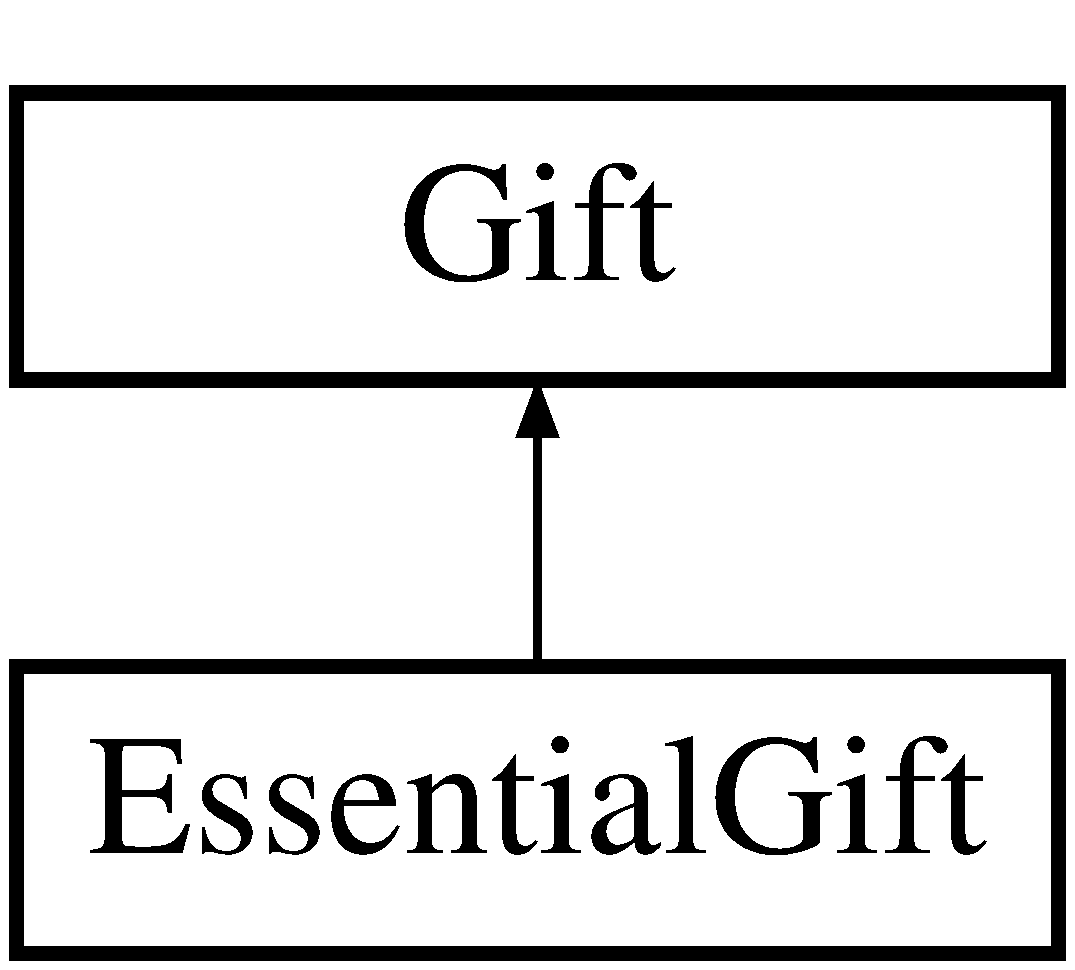
\includegraphics[height=2.000000cm]{class_essential_gift}
\end{center}
\end{figure}
\subsection*{Public Member Functions}
\begin{DoxyCompactItemize}
\item 
\hyperlink{class_essential_gift_a648490b74be632f7538144ce9c9cf704}{Essential\+Gift} (int index, int price, int value, bool taken)
\end{DoxyCompactItemize}


\subsection{Constructor \& Destructor Documentation}
\mbox{\Hypertarget{class_essential_gift_a648490b74be632f7538144ce9c9cf704}\label{class_essential_gift_a648490b74be632f7538144ce9c9cf704}} 
\index{Essential\+Gift@{Essential\+Gift}!Essential\+Gift@{Essential\+Gift}}
\index{Essential\+Gift@{Essential\+Gift}!Essential\+Gift@{Essential\+Gift}}
\subsubsection{\texorpdfstring{Essential\+Gift()}{EssentialGift()}}
{\footnotesize\ttfamily Essential\+Gift\+::\+Essential\+Gift (\begin{DoxyParamCaption}\item[{int}]{index,  }\item[{int}]{price,  }\item[{int}]{value,  }\item[{bool}]{taken }\end{DoxyParamCaption})}

Essential \hyperlink{class_gift}{Gift} constructor 

The documentation for this class was generated from the following files\+:\begin{DoxyCompactItemize}
\item 
C\+:/\+Users/\+Piyush Arora/\+Google Drive/\+Semester-\/4/\+Theory/\+I\+P\+P\+L430\+C/\+Assignment/ppl-\/assignment-\/\+Piyush\+Arora01/\+Q3 -\/ 10/Essential\+Gift.\+h\item 
C\+:/\+Users/\+Piyush Arora/\+Google Drive/\+Semester-\/4/\+Theory/\+I\+P\+P\+L430\+C/\+Assignment/ppl-\/assignment-\/\+Piyush\+Arora01/\+Q3 -\/ 10/Essential\+Gift.\+cpp\end{DoxyCompactItemize}

\hypertarget{class_gift}{}\section{Gift Class Reference}
\label{class_gift}\index{Gift@{Gift}}
\subsection*{Public Member Functions}
\begin{DoxyCompactItemize}
\item 
\hyperlink{class_gift_a3518b10b5b491f98a56e0b7d27736783}{Gift} (int price, int value)
\item 
\hyperlink{class_gift_a95ed6819ae16875595be9a0100f060de}{Gift} (int price, int value, int luxury\+Rating, int luxury\+Difficulty\+To\+Obtain)
\item 
\hyperlink{class_gift_a5f3dd07ba0552c716f3abc55d521e063}{Gift} (int price, int value, int utility\+Value, long utility\+Class)
\item 
int \hyperlink{class_gift_a999437028eda2a5aac1f3ad1c3f22cf9}{get\+Type} ()
\item 
int \hyperlink{class_gift_aa114ca9629b5f02e4df6731d33c69373}{get\+Price} ()
\item 
int \hyperlink{class_gift_aabddc4d671de70d9002461076999a574}{get\+Value} ()
\item 
int \hyperlink{class_gift_a13f625f3bf17ea98bdc61c0f824b77a4}{get\+Luxury\+Rating} ()
\item 
int \hyperlink{class_gift_aa7315f0e639d60a32c53eaaacddba937}{get\+Luxury\+Difficulty\+To\+Obtain} ()
\item 
int \hyperlink{class_gift_a109b572cc26b20b8b745b959afae678e}{get\+Utility\+Value} ()
\item 
int \hyperlink{class_gift_a16a1e01228fcd6de8fd4b607a854d2b7}{get\+Utility\+Class} ()
\item 
void \hyperlink{class_gift_a3e497fb858aade883c0b18c979963d83}{set\+Price} (int price)
\item 
void \hyperlink{class_gift_a40368c3ac78745ce67d3a2496ba3e9ce}{set\+Value} (int value)
\item 
void \hyperlink{class_gift_a40b64181f527757f46ae01441c6a73e4}{set\+Luxury\+Rating} (int luxury\+Rating)
\item 
void \hyperlink{class_gift_a6f03034c81bf5e709fd91078ef2d323b}{set\+Luxury\+Difficulty\+To\+Obtain} (int luxury\+Difficulty\+To\+Obtain)
\item 
void \hyperlink{class_gift_a3d29773a61661250ca59b63f28351d23}{set\+Utility\+Value} (int utility\+Value)
\item 
void \hyperlink{class_gift_afc8d4b95e2a9b81ddb5ccf098b217dfc}{set\+Utility\+Class} (int utility\+Class)
\end{DoxyCompactItemize}


\subsection{Constructor \& Destructor Documentation}
\mbox{\Hypertarget{class_gift_a3518b10b5b491f98a56e0b7d27736783}\label{class_gift_a3518b10b5b491f98a56e0b7d27736783}} 
\index{Gift@{Gift}!Gift@{Gift}}
\index{Gift@{Gift}!Gift@{Gift}}
\subsubsection{\texorpdfstring{Gift()}{Gift()}\hspace{0.1cm}{\footnotesize\ttfamily [1/3]}}
{\footnotesize\ttfamily Gift\+::\+Gift (\begin{DoxyParamCaption}\item[{int}]{price,  }\item[{int}]{value }\end{DoxyParamCaption})}

Create Essential \hyperlink{class_gift}{Gift} \mbox{\Hypertarget{class_gift_a95ed6819ae16875595be9a0100f060de}\label{class_gift_a95ed6819ae16875595be9a0100f060de}} 
\index{Gift@{Gift}!Gift@{Gift}}
\index{Gift@{Gift}!Gift@{Gift}}
\subsubsection{\texorpdfstring{Gift()}{Gift()}\hspace{0.1cm}{\footnotesize\ttfamily [2/3]}}
{\footnotesize\ttfamily Gift\+::\+Gift (\begin{DoxyParamCaption}\item[{int}]{price,  }\item[{int}]{value,  }\item[{int}]{luxury\+Rating,  }\item[{int}]{luxury\+Difficulty\+To\+Obtain }\end{DoxyParamCaption})}

Create Luxury \hyperlink{class_gift}{Gift} \mbox{\Hypertarget{class_gift_a5f3dd07ba0552c716f3abc55d521e063}\label{class_gift_a5f3dd07ba0552c716f3abc55d521e063}} 
\index{Gift@{Gift}!Gift@{Gift}}
\index{Gift@{Gift}!Gift@{Gift}}
\subsubsection{\texorpdfstring{Gift()}{Gift()}\hspace{0.1cm}{\footnotesize\ttfamily [3/3]}}
{\footnotesize\ttfamily Gift\+::\+Gift (\begin{DoxyParamCaption}\item[{int}]{price,  }\item[{int}]{value,  }\item[{int}]{utility\+Value,  }\item[{long}]{utility\+Class }\end{DoxyParamCaption})}

Create Utility \hyperlink{class_gift}{Gift} 

\subsection{Member Function Documentation}
\mbox{\Hypertarget{class_gift_aa7315f0e639d60a32c53eaaacddba937}\label{class_gift_aa7315f0e639d60a32c53eaaacddba937}} 
\index{Gift@{Gift}!get\+Luxury\+Difficulty\+To\+Obtain@{get\+Luxury\+Difficulty\+To\+Obtain}}
\index{get\+Luxury\+Difficulty\+To\+Obtain@{get\+Luxury\+Difficulty\+To\+Obtain}!Gift@{Gift}}
\subsubsection{\texorpdfstring{get\+Luxury\+Difficulty\+To\+Obtain()}{getLuxuryDifficultyToObtain()}}
{\footnotesize\ttfamily int Gift\+::get\+Luxury\+Difficulty\+To\+Obtain (\begin{DoxyParamCaption}{ }\end{DoxyParamCaption})}

Return Luxury Difficulty \mbox{\Hypertarget{class_gift_a13f625f3bf17ea98bdc61c0f824b77a4}\label{class_gift_a13f625f3bf17ea98bdc61c0f824b77a4}} 
\index{Gift@{Gift}!get\+Luxury\+Rating@{get\+Luxury\+Rating}}
\index{get\+Luxury\+Rating@{get\+Luxury\+Rating}!Gift@{Gift}}
\subsubsection{\texorpdfstring{get\+Luxury\+Rating()}{getLuxuryRating()}}
{\footnotesize\ttfamily int Gift\+::get\+Luxury\+Rating (\begin{DoxyParamCaption}{ }\end{DoxyParamCaption})}

Return luxury rating \mbox{\Hypertarget{class_gift_aa114ca9629b5f02e4df6731d33c69373}\label{class_gift_aa114ca9629b5f02e4df6731d33c69373}} 
\index{Gift@{Gift}!get\+Price@{get\+Price}}
\index{get\+Price@{get\+Price}!Gift@{Gift}}
\subsubsection{\texorpdfstring{get\+Price()}{getPrice()}}
{\footnotesize\ttfamily int Gift\+::get\+Price (\begin{DoxyParamCaption}{ }\end{DoxyParamCaption})}

Return gift price \mbox{\Hypertarget{class_gift_a999437028eda2a5aac1f3ad1c3f22cf9}\label{class_gift_a999437028eda2a5aac1f3ad1c3f22cf9}} 
\index{Gift@{Gift}!get\+Type@{get\+Type}}
\index{get\+Type@{get\+Type}!Gift@{Gift}}
\subsubsection{\texorpdfstring{get\+Type()}{getType()}}
{\footnotesize\ttfamily int Gift\+::get\+Type (\begin{DoxyParamCaption}{ }\end{DoxyParamCaption})}

Return gift type \mbox{\Hypertarget{class_gift_a16a1e01228fcd6de8fd4b607a854d2b7}\label{class_gift_a16a1e01228fcd6de8fd4b607a854d2b7}} 
\index{Gift@{Gift}!get\+Utility\+Class@{get\+Utility\+Class}}
\index{get\+Utility\+Class@{get\+Utility\+Class}!Gift@{Gift}}
\subsubsection{\texorpdfstring{get\+Utility\+Class()}{getUtilityClass()}}
{\footnotesize\ttfamily int Gift\+::get\+Utility\+Class (\begin{DoxyParamCaption}{ }\end{DoxyParamCaption})}

Return Utility Class \mbox{\Hypertarget{class_gift_a109b572cc26b20b8b745b959afae678e}\label{class_gift_a109b572cc26b20b8b745b959afae678e}} 
\index{Gift@{Gift}!get\+Utility\+Value@{get\+Utility\+Value}}
\index{get\+Utility\+Value@{get\+Utility\+Value}!Gift@{Gift}}
\subsubsection{\texorpdfstring{get\+Utility\+Value()}{getUtilityValue()}}
{\footnotesize\ttfamily int Gift\+::get\+Utility\+Value (\begin{DoxyParamCaption}{ }\end{DoxyParamCaption})}

Return Utility Value \mbox{\Hypertarget{class_gift_aabddc4d671de70d9002461076999a574}\label{class_gift_aabddc4d671de70d9002461076999a574}} 
\index{Gift@{Gift}!get\+Value@{get\+Value}}
\index{get\+Value@{get\+Value}!Gift@{Gift}}
\subsubsection{\texorpdfstring{get\+Value()}{getValue()}}
{\footnotesize\ttfamily int Gift\+::get\+Value (\begin{DoxyParamCaption}{ }\end{DoxyParamCaption})}

Return gift value \mbox{\Hypertarget{class_gift_a6f03034c81bf5e709fd91078ef2d323b}\label{class_gift_a6f03034c81bf5e709fd91078ef2d323b}} 
\index{Gift@{Gift}!set\+Luxury\+Difficulty\+To\+Obtain@{set\+Luxury\+Difficulty\+To\+Obtain}}
\index{set\+Luxury\+Difficulty\+To\+Obtain@{set\+Luxury\+Difficulty\+To\+Obtain}!Gift@{Gift}}
\subsubsection{\texorpdfstring{set\+Luxury\+Difficulty\+To\+Obtain()}{setLuxuryDifficultyToObtain()}}
{\footnotesize\ttfamily void Gift\+::set\+Luxury\+Difficulty\+To\+Obtain (\begin{DoxyParamCaption}\item[{int}]{luxury\+Difficulty\+To\+Obtain }\end{DoxyParamCaption})}

Set Difficulty to obtain \mbox{\Hypertarget{class_gift_a40b64181f527757f46ae01441c6a73e4}\label{class_gift_a40b64181f527757f46ae01441c6a73e4}} 
\index{Gift@{Gift}!set\+Luxury\+Rating@{set\+Luxury\+Rating}}
\index{set\+Luxury\+Rating@{set\+Luxury\+Rating}!Gift@{Gift}}
\subsubsection{\texorpdfstring{set\+Luxury\+Rating()}{setLuxuryRating()}}
{\footnotesize\ttfamily void Gift\+::set\+Luxury\+Rating (\begin{DoxyParamCaption}\item[{int}]{luxury\+Rating }\end{DoxyParamCaption})}

Set luxury rating \mbox{\Hypertarget{class_gift_a3e497fb858aade883c0b18c979963d83}\label{class_gift_a3e497fb858aade883c0b18c979963d83}} 
\index{Gift@{Gift}!set\+Price@{set\+Price}}
\index{set\+Price@{set\+Price}!Gift@{Gift}}
\subsubsection{\texorpdfstring{set\+Price()}{setPrice()}}
{\footnotesize\ttfamily void Gift\+::set\+Price (\begin{DoxyParamCaption}\item[{int}]{price }\end{DoxyParamCaption})}

Set \hyperlink{class_gift}{Gift} price \mbox{\Hypertarget{class_gift_afc8d4b95e2a9b81ddb5ccf098b217dfc}\label{class_gift_afc8d4b95e2a9b81ddb5ccf098b217dfc}} 
\index{Gift@{Gift}!set\+Utility\+Class@{set\+Utility\+Class}}
\index{set\+Utility\+Class@{set\+Utility\+Class}!Gift@{Gift}}
\subsubsection{\texorpdfstring{set\+Utility\+Class()}{setUtilityClass()}}
{\footnotesize\ttfamily void Gift\+::set\+Utility\+Class (\begin{DoxyParamCaption}\item[{int}]{utility\+Class }\end{DoxyParamCaption})}

Set utility class \mbox{\Hypertarget{class_gift_a3d29773a61661250ca59b63f28351d23}\label{class_gift_a3d29773a61661250ca59b63f28351d23}} 
\index{Gift@{Gift}!set\+Utility\+Value@{set\+Utility\+Value}}
\index{set\+Utility\+Value@{set\+Utility\+Value}!Gift@{Gift}}
\subsubsection{\texorpdfstring{set\+Utility\+Value()}{setUtilityValue()}}
{\footnotesize\ttfamily void Gift\+::set\+Utility\+Value (\begin{DoxyParamCaption}\item[{int}]{utility\+Value }\end{DoxyParamCaption})}

Set utility value \mbox{\Hypertarget{class_gift_a40368c3ac78745ce67d3a2496ba3e9ce}\label{class_gift_a40368c3ac78745ce67d3a2496ba3e9ce}} 
\index{Gift@{Gift}!set\+Value@{set\+Value}}
\index{set\+Value@{set\+Value}!Gift@{Gift}}
\subsubsection{\texorpdfstring{set\+Value()}{setValue()}}
{\footnotesize\ttfamily void Gift\+::set\+Value (\begin{DoxyParamCaption}\item[{int}]{value }\end{DoxyParamCaption})}

Set \hyperlink{class_gift}{Gift} value 

The documentation for this class was generated from the following files\+:\begin{DoxyCompactItemize}
\item 
C\+:/\+Users/\+Piyush Arora/\+Google Drive/\+Semester-\/4/\+Theory/\+I\+P\+P\+L430\+C/\+Assignment/Gift.\+h\item 
C\+:/\+Users/\+Piyush Arora/\+Google Drive/\+Semester-\/4/\+Theory/\+I\+P\+P\+L430\+C/\+Assignment/Gift.\+cpp\end{DoxyCompactItemize}

\hypertarget{class_girl}{}\section{Girl Class Reference}
\label{class_girl}\index{Girl@{Girl}}
\subsection*{Public Member Functions}
\begin{DoxyCompactItemize}
\item 
\hyperlink{class_girl_a1a8fcd5a2b2d09ad68b8d987a42820fa}{Girl} (std\+::string name, int attractiveness, int maintenance\+Cost, int intelligence\+Level, int type, int boy\+Choice)
\item 
std\+::string \hyperlink{class_girl_a27a705fb94b92dfd6929d0bf4bcaf5e1}{get\+Name} ()
\item 
int \hyperlink{class_girl_a04cfe3e0c21240f92c19152630a40252}{get\+Attractiveness} ()
\item 
int \hyperlink{class_girl_a8fa9751cb04f9c510a635c9f19a1d4d9}{get\+Maintenance\+Cost} ()
\item 
int \hyperlink{class_girl_a8b9ea4f67c0e682f65fb683f1c1ee766}{get\+Intelligence\+Level} ()
\item 
bool \hyperlink{class_girl_ac4768f02f66b1d124fa7da9c0d85a078}{is\+Committed} ()
\item 
std\+::string \hyperlink{class_girl_a532906e2a807138de027b2a822e91abd}{get\+Partner} ()
\item 
int \hyperlink{class_girl_acd2e75d7212ce1223945c6befff293b8}{get\+Type} ()
\item 
int \hyperlink{class_girl_a23ed372fae6fc44694d5ffa39fa455cb}{get\+Boy\+Choice} ()
\item 
double \hyperlink{class_girl_adf0956456e02324db90c009c0c3c47d3}{get\+Happiness} ()
\item 
void \hyperlink{class_girl_a8b94b6e5b0ebe961040e1c1033832588}{set\+Attractiveness} (int attractiveness)
\item 
void \hyperlink{class_girl_a585d7b2bbaec1d608e64fd29138e4632}{set\+Maintenance\+Cost} (int maintenance\+Cost)
\item 
void \hyperlink{class_girl_a7f02a69fc79e52b46161ed49f8901ecd}{set\+Committed} (bool committed)
\item 
void \hyperlink{class_girl_aeeb035a49f221a0ba3744b35e26fba3f}{set\+Intelligence\+Level} (int intelligence\+Level)
\item 
void \hyperlink{class_girl_a4f75b05e9d1362c27053248521e118be}{set\+Partner} (std\+::string partner)
\item 
void \hyperlink{class_girl_ac83625dfc5d32ef2ea53714613926c49}{set\+Type} (int type)
\item 
void \hyperlink{class_girl_a786c96c2084a8571ee04b1b38b4eb357}{set\+Happiness} (double happiness)
\item 
void \hyperlink{class_girl_a48efb2fda11ce41c74511be3bfc2510c}{set\+Boy\+Choice} (int boy\+Choice)
\end{DoxyCompactItemize}


\subsection{Constructor \& Destructor Documentation}
\mbox{\Hypertarget{class_girl_a1a8fcd5a2b2d09ad68b8d987a42820fa}\label{class_girl_a1a8fcd5a2b2d09ad68b8d987a42820fa}} 
\index{Girl@{Girl}!Girl@{Girl}}
\index{Girl@{Girl}!Girl@{Girl}}
\subsubsection{\texorpdfstring{Girl()}{Girl()}}
{\footnotesize\ttfamily Girl\+::\+Girl (\begin{DoxyParamCaption}\item[{std\+::string}]{name,  }\item[{int}]{attractiveness,  }\item[{int}]{maintenance\+Cost,  }\item[{int}]{intelligence\+Level,  }\item[{int}]{type,  }\item[{int}]{boy\+Choice }\end{DoxyParamCaption})}

\hyperlink{class_girl}{Girl} constructor 

\subsection{Member Function Documentation}
\mbox{\Hypertarget{class_girl_a04cfe3e0c21240f92c19152630a40252}\label{class_girl_a04cfe3e0c21240f92c19152630a40252}} 
\index{Girl@{Girl}!get\+Attractiveness@{get\+Attractiveness}}
\index{get\+Attractiveness@{get\+Attractiveness}!Girl@{Girl}}
\subsubsection{\texorpdfstring{get\+Attractiveness()}{getAttractiveness()}}
{\footnotesize\ttfamily int Girl\+::get\+Attractiveness (\begin{DoxyParamCaption}{ }\end{DoxyParamCaption})}

Return girl attractiveness \mbox{\Hypertarget{class_girl_a23ed372fae6fc44694d5ffa39fa455cb}\label{class_girl_a23ed372fae6fc44694d5ffa39fa455cb}} 
\index{Girl@{Girl}!get\+Boy\+Choice@{get\+Boy\+Choice}}
\index{get\+Boy\+Choice@{get\+Boy\+Choice}!Girl@{Girl}}
\subsubsection{\texorpdfstring{get\+Boy\+Choice()}{getBoyChoice()}}
{\footnotesize\ttfamily int Girl\+::get\+Boy\+Choice (\begin{DoxyParamCaption}{ }\end{DoxyParamCaption})}

Return her boy\textquotesingle{}s choice \mbox{\Hypertarget{class_girl_adf0956456e02324db90c009c0c3c47d3}\label{class_girl_adf0956456e02324db90c009c0c3c47d3}} 
\index{Girl@{Girl}!get\+Happiness@{get\+Happiness}}
\index{get\+Happiness@{get\+Happiness}!Girl@{Girl}}
\subsubsection{\texorpdfstring{get\+Happiness()}{getHappiness()}}
{\footnotesize\ttfamily double Girl\+::get\+Happiness (\begin{DoxyParamCaption}{ }\end{DoxyParamCaption})}

Return gir\textquotesingle{}s happiness \mbox{\Hypertarget{class_girl_a8b9ea4f67c0e682f65fb683f1c1ee766}\label{class_girl_a8b9ea4f67c0e682f65fb683f1c1ee766}} 
\index{Girl@{Girl}!get\+Intelligence\+Level@{get\+Intelligence\+Level}}
\index{get\+Intelligence\+Level@{get\+Intelligence\+Level}!Girl@{Girl}}
\subsubsection{\texorpdfstring{get\+Intelligence\+Level()}{getIntelligenceLevel()}}
{\footnotesize\ttfamily int Girl\+::get\+Intelligence\+Level (\begin{DoxyParamCaption}{ }\end{DoxyParamCaption})}

Return gir\textquotesingle{}s intelligence level \mbox{\Hypertarget{class_girl_a8fa9751cb04f9c510a635c9f19a1d4d9}\label{class_girl_a8fa9751cb04f9c510a635c9f19a1d4d9}} 
\index{Girl@{Girl}!get\+Maintenance\+Cost@{get\+Maintenance\+Cost}}
\index{get\+Maintenance\+Cost@{get\+Maintenance\+Cost}!Girl@{Girl}}
\subsubsection{\texorpdfstring{get\+Maintenance\+Cost()}{getMaintenanceCost()}}
{\footnotesize\ttfamily int Girl\+::get\+Maintenance\+Cost (\begin{DoxyParamCaption}{ }\end{DoxyParamCaption})}

Return girl\textquotesingle{}s maintenance cost \mbox{\Hypertarget{class_girl_a27a705fb94b92dfd6929d0bf4bcaf5e1}\label{class_girl_a27a705fb94b92dfd6929d0bf4bcaf5e1}} 
\index{Girl@{Girl}!get\+Name@{get\+Name}}
\index{get\+Name@{get\+Name}!Girl@{Girl}}
\subsubsection{\texorpdfstring{get\+Name()}{getName()}}
{\footnotesize\ttfamily std\+::string Girl\+::get\+Name (\begin{DoxyParamCaption}{ }\end{DoxyParamCaption})}

Return girl name \mbox{\Hypertarget{class_girl_a532906e2a807138de027b2a822e91abd}\label{class_girl_a532906e2a807138de027b2a822e91abd}} 
\index{Girl@{Girl}!get\+Partner@{get\+Partner}}
\index{get\+Partner@{get\+Partner}!Girl@{Girl}}
\subsubsection{\texorpdfstring{get\+Partner()}{getPartner()}}
{\footnotesize\ttfamily std\+::string Girl\+::get\+Partner (\begin{DoxyParamCaption}{ }\end{DoxyParamCaption})}

Return her partner \mbox{\Hypertarget{class_girl_acd2e75d7212ce1223945c6befff293b8}\label{class_girl_acd2e75d7212ce1223945c6befff293b8}} 
\index{Girl@{Girl}!get\+Type@{get\+Type}}
\index{get\+Type@{get\+Type}!Girl@{Girl}}
\subsubsection{\texorpdfstring{get\+Type()}{getType()}}
{\footnotesize\ttfamily int Girl\+::get\+Type (\begin{DoxyParamCaption}{ }\end{DoxyParamCaption})}

Return her type \mbox{\Hypertarget{class_girl_ac4768f02f66b1d124fa7da9c0d85a078}\label{class_girl_ac4768f02f66b1d124fa7da9c0d85a078}} 
\index{Girl@{Girl}!is\+Committed@{is\+Committed}}
\index{is\+Committed@{is\+Committed}!Girl@{Girl}}
\subsubsection{\texorpdfstring{is\+Committed()}{isCommitted()}}
{\footnotesize\ttfamily bool Girl\+::is\+Committed (\begin{DoxyParamCaption}{ }\end{DoxyParamCaption})}

Return committed status \mbox{\Hypertarget{class_girl_a8b94b6e5b0ebe961040e1c1033832588}\label{class_girl_a8b94b6e5b0ebe961040e1c1033832588}} 
\index{Girl@{Girl}!set\+Attractiveness@{set\+Attractiveness}}
\index{set\+Attractiveness@{set\+Attractiveness}!Girl@{Girl}}
\subsubsection{\texorpdfstring{set\+Attractiveness()}{setAttractiveness()}}
{\footnotesize\ttfamily void Girl\+::set\+Attractiveness (\begin{DoxyParamCaption}\item[{int}]{attractiveness }\end{DoxyParamCaption})}

Set attractiveness \mbox{\Hypertarget{class_girl_a48efb2fda11ce41c74511be3bfc2510c}\label{class_girl_a48efb2fda11ce41c74511be3bfc2510c}} 
\index{Girl@{Girl}!set\+Boy\+Choice@{set\+Boy\+Choice}}
\index{set\+Boy\+Choice@{set\+Boy\+Choice}!Girl@{Girl}}
\subsubsection{\texorpdfstring{set\+Boy\+Choice()}{setBoyChoice()}}
{\footnotesize\ttfamily void Girl\+::set\+Boy\+Choice (\begin{DoxyParamCaption}\item[{int}]{boy\+Choice }\end{DoxyParamCaption})}

Set her boy preference

Boy\+Choice = 0 =$>$ Most attractive; Boy\+Choice = 1 =$>$ Most rich; Boy\+Choice = 2 =$>$ Most intelligent; ! \mbox{\Hypertarget{class_girl_a7f02a69fc79e52b46161ed49f8901ecd}\label{class_girl_a7f02a69fc79e52b46161ed49f8901ecd}} 
\index{Girl@{Girl}!set\+Committed@{set\+Committed}}
\index{set\+Committed@{set\+Committed}!Girl@{Girl}}
\subsubsection{\texorpdfstring{set\+Committed()}{setCommitted()}}
{\footnotesize\ttfamily void Girl\+::set\+Committed (\begin{DoxyParamCaption}\item[{bool}]{committed }\end{DoxyParamCaption})}

Set commited status \mbox{\Hypertarget{class_girl_a786c96c2084a8571ee04b1b38b4eb357}\label{class_girl_a786c96c2084a8571ee04b1b38b4eb357}} 
\index{Girl@{Girl}!set\+Happiness@{set\+Happiness}}
\index{set\+Happiness@{set\+Happiness}!Girl@{Girl}}
\subsubsection{\texorpdfstring{set\+Happiness()}{setHappiness()}}
{\footnotesize\ttfamily void Girl\+::set\+Happiness (\begin{DoxyParamCaption}\item[{double}]{happiness }\end{DoxyParamCaption})}

Set her happiness \mbox{\Hypertarget{class_girl_aeeb035a49f221a0ba3744b35e26fba3f}\label{class_girl_aeeb035a49f221a0ba3744b35e26fba3f}} 
\index{Girl@{Girl}!set\+Intelligence\+Level@{set\+Intelligence\+Level}}
\index{set\+Intelligence\+Level@{set\+Intelligence\+Level}!Girl@{Girl}}
\subsubsection{\texorpdfstring{set\+Intelligence\+Level()}{setIntelligenceLevel()}}
{\footnotesize\ttfamily void Girl\+::set\+Intelligence\+Level (\begin{DoxyParamCaption}\item[{int}]{intelligence\+Level }\end{DoxyParamCaption})}

Set intelligence level \mbox{\Hypertarget{class_girl_a585d7b2bbaec1d608e64fd29138e4632}\label{class_girl_a585d7b2bbaec1d608e64fd29138e4632}} 
\index{Girl@{Girl}!set\+Maintenance\+Cost@{set\+Maintenance\+Cost}}
\index{set\+Maintenance\+Cost@{set\+Maintenance\+Cost}!Girl@{Girl}}
\subsubsection{\texorpdfstring{set\+Maintenance\+Cost()}{setMaintenanceCost()}}
{\footnotesize\ttfamily void Girl\+::set\+Maintenance\+Cost (\begin{DoxyParamCaption}\item[{int}]{maintenance\+Cost }\end{DoxyParamCaption})}

Set maintenance cost \mbox{\Hypertarget{class_girl_a4f75b05e9d1362c27053248521e118be}\label{class_girl_a4f75b05e9d1362c27053248521e118be}} 
\index{Girl@{Girl}!set\+Partner@{set\+Partner}}
\index{set\+Partner@{set\+Partner}!Girl@{Girl}}
\subsubsection{\texorpdfstring{set\+Partner()}{setPartner()}}
{\footnotesize\ttfamily void Girl\+::set\+Partner (\begin{DoxyParamCaption}\item[{std\+::string}]{partner }\end{DoxyParamCaption})}

Set partner \mbox{\Hypertarget{class_girl_ac83625dfc5d32ef2ea53714613926c49}\label{class_girl_ac83625dfc5d32ef2ea53714613926c49}} 
\index{Girl@{Girl}!set\+Type@{set\+Type}}
\index{set\+Type@{set\+Type}!Girl@{Girl}}
\subsubsection{\texorpdfstring{set\+Type()}{setType()}}
{\footnotesize\ttfamily void Girl\+::set\+Type (\begin{DoxyParamCaption}\item[{int}]{type }\end{DoxyParamCaption})}

Set type of girl

Type = 0 =$>$ Choosy; Type = 1 =$>$ Normal; Type = 2 =$>$ Desperate; ! 

The documentation for this class was generated from the following files\+:\begin{DoxyCompactItemize}
\item 
C\+:/\+Users/\+Piyush Arora/\+Google Drive/\+Semester-\/4/\+Theory/\+I\+P\+P\+L430\+C/\+Assignment/Girl.\+h\item 
C\+:/\+Users/\+Piyush Arora/\+Google Drive/\+Semester-\/4/\+Theory/\+I\+P\+P\+L430\+C/\+Assignment/Girl.\+cpp\end{DoxyCompactItemize}

\hypertarget{class_luxury_gift}{}\section{Luxury\+Gift Class Reference}
\label{class_luxury_gift}\index{Luxury\+Gift@{Luxury\+Gift}}
Inheritance diagram for Luxury\+Gift\+:\begin{figure}[H]
\begin{center}
\leavevmode
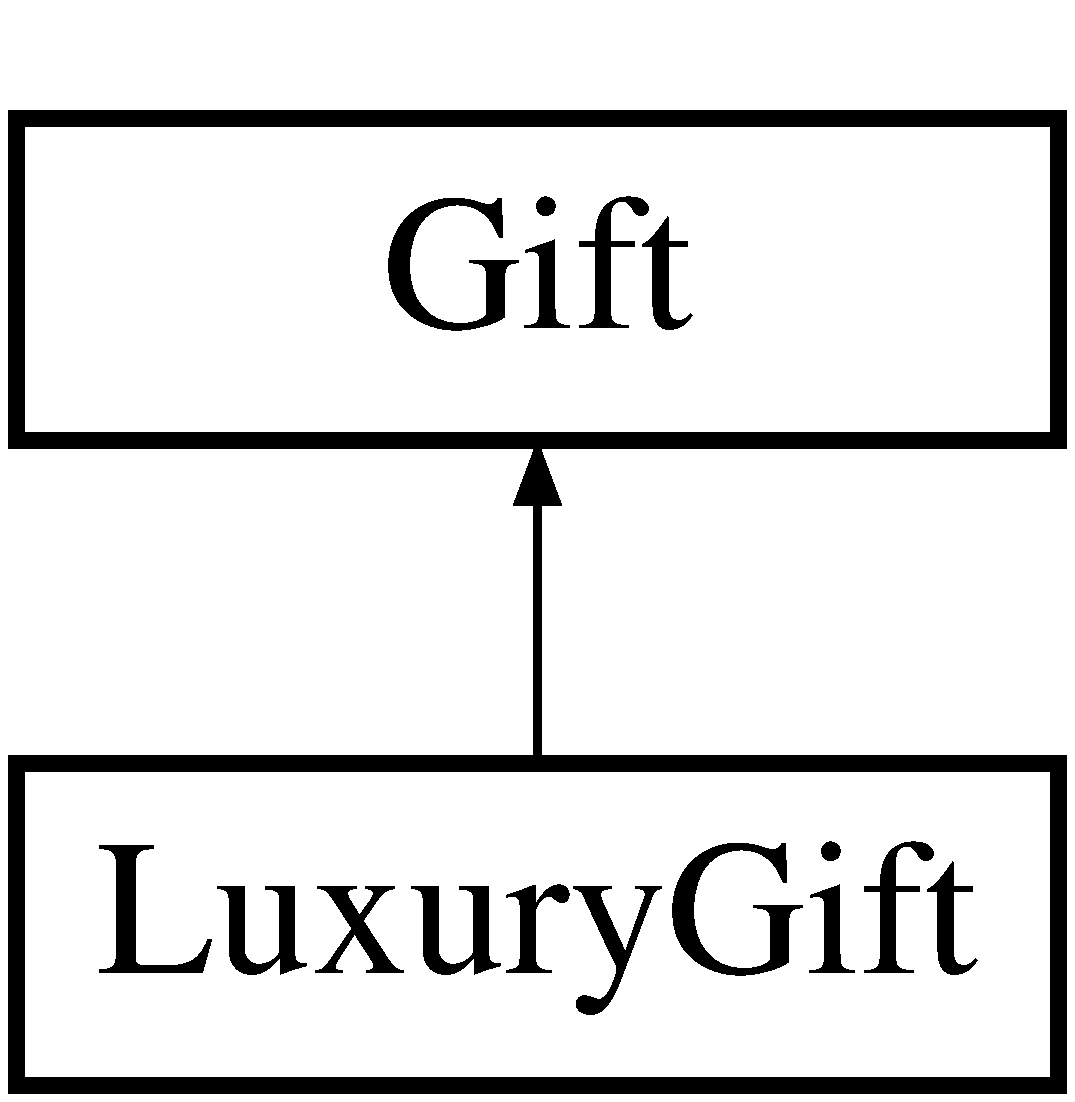
\includegraphics[height=2.000000cm]{class_luxury_gift}
\end{center}
\end{figure}
\subsection*{Public Member Functions}
\begin{DoxyCompactItemize}
\item 
\hyperlink{class_luxury_gift_ac4a20f9cde3d296abbaf2cda06318ff0}{Luxury\+Gift} (int index, int price, int value, bool taken, int luxury\+Rating, int luxury\+Difficulty\+To\+Obtain)
\item 
int \hyperlink{class_luxury_gift_a7f1f89000bc9a5c2c88d525dc8f7f3c2}{get\+Luxury\+Rating} ()
\item 
int \hyperlink{class_luxury_gift_a6441f2a7863c9079ce153721d3b6bce6}{get\+Luxury\+Difficulty\+To\+Obtain} ()
\item 
void \hyperlink{class_luxury_gift_a3a2f57732502c45b2e5bcab6963d4de7}{set\+Luxury\+Rating} (int luxury\+Rating)
\item 
void \hyperlink{class_luxury_gift_ab7897f54cd7a896dad198107e92fb8ca}{set\+Luxury\+Difficulty\+To\+Obtain} (int luxury\+Difficulty\+To\+Obtain)
\end{DoxyCompactItemize}


\subsection{Constructor \& Destructor Documentation}
\mbox{\Hypertarget{class_luxury_gift_ac4a20f9cde3d296abbaf2cda06318ff0}\label{class_luxury_gift_ac4a20f9cde3d296abbaf2cda06318ff0}} 
\index{Luxury\+Gift@{Luxury\+Gift}!Luxury\+Gift@{Luxury\+Gift}}
\index{Luxury\+Gift@{Luxury\+Gift}!Luxury\+Gift@{Luxury\+Gift}}
\subsubsection{\texorpdfstring{Luxury\+Gift()}{LuxuryGift()}}
{\footnotesize\ttfamily Luxury\+Gift\+::\+Luxury\+Gift (\begin{DoxyParamCaption}\item[{int}]{index,  }\item[{int}]{price,  }\item[{int}]{value,  }\item[{bool}]{taken,  }\item[{int}]{luxury\+Rating,  }\item[{int}]{luxury\+Difficulty\+To\+Obtain }\end{DoxyParamCaption})}

Luxury \hyperlink{class_gift}{Gift} constructor 

\subsection{Member Function Documentation}
\mbox{\Hypertarget{class_luxury_gift_a6441f2a7863c9079ce153721d3b6bce6}\label{class_luxury_gift_a6441f2a7863c9079ce153721d3b6bce6}} 
\index{Luxury\+Gift@{Luxury\+Gift}!get\+Luxury\+Difficulty\+To\+Obtain@{get\+Luxury\+Difficulty\+To\+Obtain}}
\index{get\+Luxury\+Difficulty\+To\+Obtain@{get\+Luxury\+Difficulty\+To\+Obtain}!Luxury\+Gift@{Luxury\+Gift}}
\subsubsection{\texorpdfstring{get\+Luxury\+Difficulty\+To\+Obtain()}{getLuxuryDifficultyToObtain()}}
{\footnotesize\ttfamily int Luxury\+Gift\+::get\+Luxury\+Difficulty\+To\+Obtain (\begin{DoxyParamCaption}{ }\end{DoxyParamCaption})}

Return Luxury Difficulty \mbox{\Hypertarget{class_luxury_gift_a7f1f89000bc9a5c2c88d525dc8f7f3c2}\label{class_luxury_gift_a7f1f89000bc9a5c2c88d525dc8f7f3c2}} 
\index{Luxury\+Gift@{Luxury\+Gift}!get\+Luxury\+Rating@{get\+Luxury\+Rating}}
\index{get\+Luxury\+Rating@{get\+Luxury\+Rating}!Luxury\+Gift@{Luxury\+Gift}}
\subsubsection{\texorpdfstring{get\+Luxury\+Rating()}{getLuxuryRating()}}
{\footnotesize\ttfamily int Luxury\+Gift\+::get\+Luxury\+Rating (\begin{DoxyParamCaption}{ }\end{DoxyParamCaption})}

Return luxury rating \mbox{\Hypertarget{class_luxury_gift_ab7897f54cd7a896dad198107e92fb8ca}\label{class_luxury_gift_ab7897f54cd7a896dad198107e92fb8ca}} 
\index{Luxury\+Gift@{Luxury\+Gift}!set\+Luxury\+Difficulty\+To\+Obtain@{set\+Luxury\+Difficulty\+To\+Obtain}}
\index{set\+Luxury\+Difficulty\+To\+Obtain@{set\+Luxury\+Difficulty\+To\+Obtain}!Luxury\+Gift@{Luxury\+Gift}}
\subsubsection{\texorpdfstring{set\+Luxury\+Difficulty\+To\+Obtain()}{setLuxuryDifficultyToObtain()}}
{\footnotesize\ttfamily void Luxury\+Gift\+::set\+Luxury\+Difficulty\+To\+Obtain (\begin{DoxyParamCaption}\item[{int}]{luxury\+Difficulty\+To\+Obtain }\end{DoxyParamCaption})}

Set Difficulty to obtain \mbox{\Hypertarget{class_luxury_gift_a3a2f57732502c45b2e5bcab6963d4de7}\label{class_luxury_gift_a3a2f57732502c45b2e5bcab6963d4de7}} 
\index{Luxury\+Gift@{Luxury\+Gift}!set\+Luxury\+Rating@{set\+Luxury\+Rating}}
\index{set\+Luxury\+Rating@{set\+Luxury\+Rating}!Luxury\+Gift@{Luxury\+Gift}}
\subsubsection{\texorpdfstring{set\+Luxury\+Rating()}{setLuxuryRating()}}
{\footnotesize\ttfamily void Luxury\+Gift\+::set\+Luxury\+Rating (\begin{DoxyParamCaption}\item[{int}]{luxury\+Rating }\end{DoxyParamCaption})}

Set luxury rating 

The documentation for this class was generated from the following files\+:\begin{DoxyCompactItemize}
\item 
C\+:/\+Users/\+Piyush Arora/\+Google Drive/\+Semester-\/4/\+Theory/\+I\+P\+P\+L430\+C/\+Assignment/ppl-\/assignment-\/\+Piyush\+Arora01/\+Q3 -\/ 10/Luxury\+Gift.\+h\item 
C\+:/\+Users/\+Piyush Arora/\+Google Drive/\+Semester-\/4/\+Theory/\+I\+P\+P\+L430\+C/\+Assignment/ppl-\/assignment-\/\+Piyush\+Arora01/\+Q3 -\/ 10/Luxury\+Gift.\+cpp\end{DoxyCompactItemize}

\hypertarget{class_person}{}\section{Person Class Reference}
\label{class_person}\index{Person@{Person}}
Inheritance diagram for Person\+:\begin{figure}[H]
\begin{center}
\leavevmode
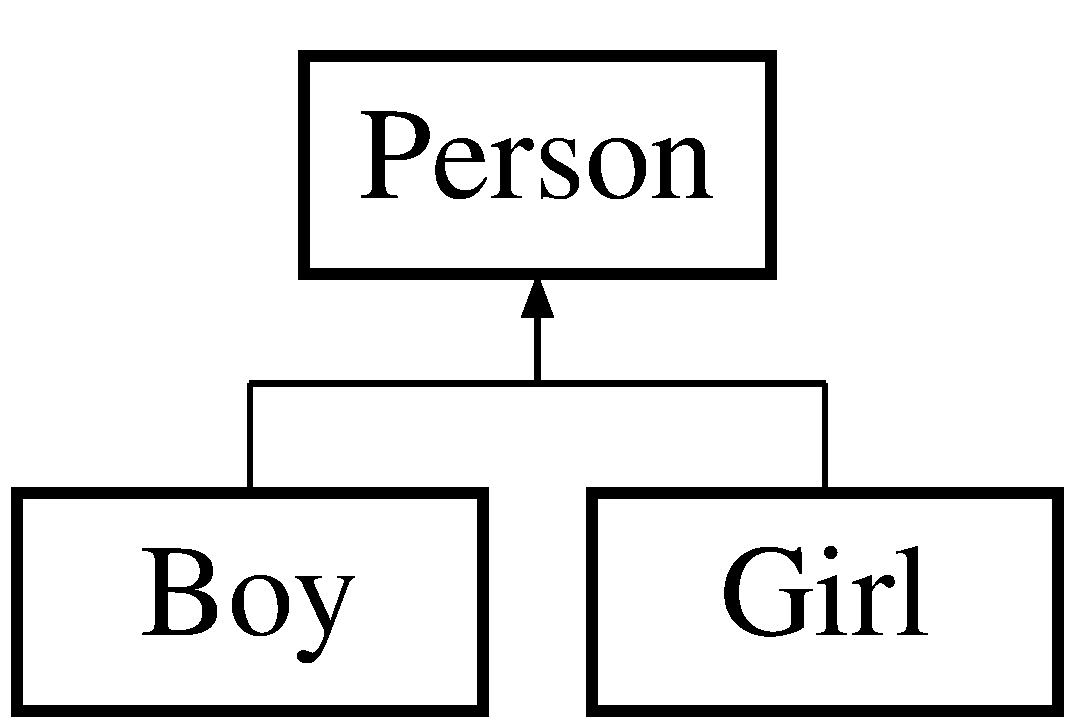
\includegraphics[height=2.000000cm]{class_person}
\end{center}
\end{figure}
\subsection*{Public Member Functions}
\begin{DoxyCompactItemize}
\item 
\mbox{\Hypertarget{class_person_adb2544355d4e11633c99388d1b7bfd12}\label{class_person_adb2544355d4e11633c99388d1b7bfd12}} 
{\bfseries Person} (int index, std\+::string name, int attractiveness, int intelligence\+Level, int type)
\item 
std\+::string \hyperlink{class_person_ae1a03b01b79596d533e63c0a866e2525}{get\+Name} ()
\item 
int \hyperlink{class_person_ac75bad62721ee53f0e765353984e1290}{get\+Index} ()
\item 
int \hyperlink{class_person_a5d9004521f0591b18c07e69423274714}{get\+Attractiveness} ()
\item 
int \hyperlink{class_person_ac3fcb86ca37de466997783e1f60080a3}{get\+Intelligence\+Level} ()
\item 
bool \hyperlink{class_person_a05b6e810e9bbf95d5346a18082e9d799}{is\+Committed} ()
\item 
int \hyperlink{class_person_a5c653289ac6e18bb1b588c688f39430a}{get\+Type} ()
\item 
void \hyperlink{class_person_a26236ea8f9fbc4171df210edd6ccd2ea}{set\+Attractiveness} (int attractiveness)
\item 
void \hyperlink{class_person_a96d58d6da36c25c246ae0fc9370084d2}{set\+Committed} (bool committed)
\item 
void \hyperlink{class_person_ac8633ca29c81c39e8aed74992633c720}{set\+Intelligence\+Level} (int intelligence\+Level)
\item 
void \hyperlink{class_person_a02b0a78cc72c4808785c6e390bd06946}{set\+Type} (int type)
\end{DoxyCompactItemize}


\subsection{Member Function Documentation}
\mbox{\Hypertarget{class_person_a5d9004521f0591b18c07e69423274714}\label{class_person_a5d9004521f0591b18c07e69423274714}} 
\index{Person@{Person}!get\+Attractiveness@{get\+Attractiveness}}
\index{get\+Attractiveness@{get\+Attractiveness}!Person@{Person}}
\subsubsection{\texorpdfstring{get\+Attractiveness()}{getAttractiveness()}}
{\footnotesize\ttfamily int Person\+::get\+Attractiveness (\begin{DoxyParamCaption}{ }\end{DoxyParamCaption})}

Return person attractiveness \mbox{\Hypertarget{class_person_ac75bad62721ee53f0e765353984e1290}\label{class_person_ac75bad62721ee53f0e765353984e1290}} 
\index{Person@{Person}!get\+Index@{get\+Index}}
\index{get\+Index@{get\+Index}!Person@{Person}}
\subsubsection{\texorpdfstring{get\+Index()}{getIndex()}}
{\footnotesize\ttfamily int Person\+::get\+Index (\begin{DoxyParamCaption}{ }\end{DoxyParamCaption})}

Return person\textquotesingle{}s index \mbox{\Hypertarget{class_person_ac3fcb86ca37de466997783e1f60080a3}\label{class_person_ac3fcb86ca37de466997783e1f60080a3}} 
\index{Person@{Person}!get\+Intelligence\+Level@{get\+Intelligence\+Level}}
\index{get\+Intelligence\+Level@{get\+Intelligence\+Level}!Person@{Person}}
\subsubsection{\texorpdfstring{get\+Intelligence\+Level()}{getIntelligenceLevel()}}
{\footnotesize\ttfamily int Person\+::get\+Intelligence\+Level (\begin{DoxyParamCaption}{ }\end{DoxyParamCaption})}

Return gir\textquotesingle{}s intelligence level \mbox{\Hypertarget{class_person_ae1a03b01b79596d533e63c0a866e2525}\label{class_person_ae1a03b01b79596d533e63c0a866e2525}} 
\index{Person@{Person}!get\+Name@{get\+Name}}
\index{get\+Name@{get\+Name}!Person@{Person}}
\subsubsection{\texorpdfstring{get\+Name()}{getName()}}
{\footnotesize\ttfamily std\+::string Person\+::get\+Name (\begin{DoxyParamCaption}{ }\end{DoxyParamCaption})}

Return person name \mbox{\Hypertarget{class_person_a5c653289ac6e18bb1b588c688f39430a}\label{class_person_a5c653289ac6e18bb1b588c688f39430a}} 
\index{Person@{Person}!get\+Type@{get\+Type}}
\index{get\+Type@{get\+Type}!Person@{Person}}
\subsubsection{\texorpdfstring{get\+Type()}{getType()}}
{\footnotesize\ttfamily int Person\+::get\+Type (\begin{DoxyParamCaption}{ }\end{DoxyParamCaption})}

Return type

\begin{DoxyVerb}BOY:
    Type = 0 => Miser;
    Type = 1 => Generous;
    Type = 2 => Geeks;
GIRL:
    Type = 0 => Choosy;
    Type = 1 => Normal;
    Type = 2 => Desperate;
\end{DoxyVerb}
 ! \mbox{\Hypertarget{class_person_a05b6e810e9bbf95d5346a18082e9d799}\label{class_person_a05b6e810e9bbf95d5346a18082e9d799}} 
\index{Person@{Person}!is\+Committed@{is\+Committed}}
\index{is\+Committed@{is\+Committed}!Person@{Person}}
\subsubsection{\texorpdfstring{is\+Committed()}{isCommitted()}}
{\footnotesize\ttfamily bool Person\+::is\+Committed (\begin{DoxyParamCaption}{ }\end{DoxyParamCaption})}

Return committed status \mbox{\Hypertarget{class_person_a26236ea8f9fbc4171df210edd6ccd2ea}\label{class_person_a26236ea8f9fbc4171df210edd6ccd2ea}} 
\index{Person@{Person}!set\+Attractiveness@{set\+Attractiveness}}
\index{set\+Attractiveness@{set\+Attractiveness}!Person@{Person}}
\subsubsection{\texorpdfstring{set\+Attractiveness()}{setAttractiveness()}}
{\footnotesize\ttfamily void Person\+::set\+Attractiveness (\begin{DoxyParamCaption}\item[{int}]{attractiveness }\end{DoxyParamCaption})}

Set attractiveness \mbox{\Hypertarget{class_person_a96d58d6da36c25c246ae0fc9370084d2}\label{class_person_a96d58d6da36c25c246ae0fc9370084d2}} 
\index{Person@{Person}!set\+Committed@{set\+Committed}}
\index{set\+Committed@{set\+Committed}!Person@{Person}}
\subsubsection{\texorpdfstring{set\+Committed()}{setCommitted()}}
{\footnotesize\ttfamily void Person\+::set\+Committed (\begin{DoxyParamCaption}\item[{bool}]{committed }\end{DoxyParamCaption})}

Set commited status \mbox{\Hypertarget{class_person_ac8633ca29c81c39e8aed74992633c720}\label{class_person_ac8633ca29c81c39e8aed74992633c720}} 
\index{Person@{Person}!set\+Intelligence\+Level@{set\+Intelligence\+Level}}
\index{set\+Intelligence\+Level@{set\+Intelligence\+Level}!Person@{Person}}
\subsubsection{\texorpdfstring{set\+Intelligence\+Level()}{setIntelligenceLevel()}}
{\footnotesize\ttfamily void Person\+::set\+Intelligence\+Level (\begin{DoxyParamCaption}\item[{int}]{intelligence\+Level }\end{DoxyParamCaption})}

Set intelligence level \mbox{\Hypertarget{class_person_a02b0a78cc72c4808785c6e390bd06946}\label{class_person_a02b0a78cc72c4808785c6e390bd06946}} 
\index{Person@{Person}!set\+Type@{set\+Type}}
\index{set\+Type@{set\+Type}!Person@{Person}}
\subsubsection{\texorpdfstring{set\+Type()}{setType()}}
{\footnotesize\ttfamily void Person\+::set\+Type (\begin{DoxyParamCaption}\item[{int}]{type }\end{DoxyParamCaption})}

Set person type 

The documentation for this class was generated from the following files\+:\begin{DoxyCompactItemize}
\item 
C\+:/\+Users/\+Piyush Arora/\+Google Drive/\+Semester-\/4/\+Theory/\+I\+P\+P\+L430\+C/\+Assignment/ppl-\/assignment-\/\+Piyush\+Arora01/\+Q3 -\/ 10/Person.\+h\item 
C\+:/\+Users/\+Piyush Arora/\+Google Drive/\+Semester-\/4/\+Theory/\+I\+P\+P\+L430\+C/\+Assignment/ppl-\/assignment-\/\+Piyush\+Arora01/\+Q3 -\/ 10/Person.\+cpp\end{DoxyCompactItemize}

\hypertarget{class_utility_gift}{}\section{Utility\+Gift Class Reference}
\label{class_utility_gift}\index{Utility\+Gift@{Utility\+Gift}}
Inheritance diagram for Utility\+Gift\+:\begin{figure}[H]
\begin{center}
\leavevmode
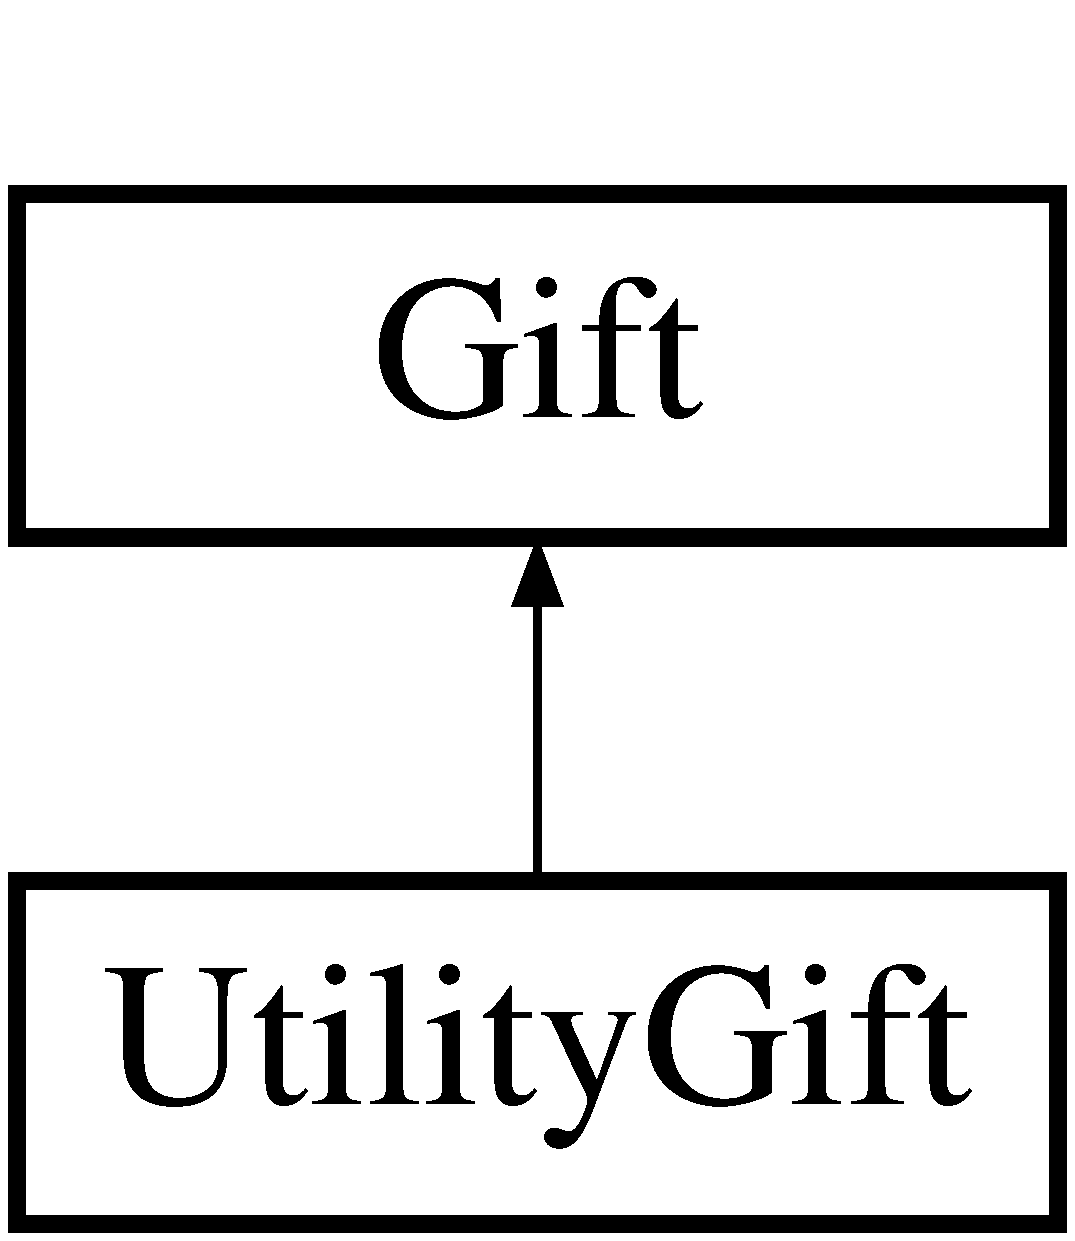
\includegraphics[height=2.000000cm]{class_utility_gift}
\end{center}
\end{figure}
\subsection*{Public Member Functions}
\begin{DoxyCompactItemize}
\item 
\hyperlink{class_utility_gift_a59535bee63b46cdf9973a2a986829736}{Utility\+Gift} (int index, int price, int value, bool taken, int utility\+Value, int utility\+Class)
\item 
int \hyperlink{class_utility_gift_ad40c77a46869bdedc03de940ff64e42e}{get\+Utility\+Value} ()
\item 
int \hyperlink{class_utility_gift_a6a7f37fde70bb92718d6c0b751a092c5}{get\+Utility\+Class} ()
\item 
void \hyperlink{class_utility_gift_a7dbd7e650be49d1f4e28b16b9a78a4c7}{set\+Utility\+Value} (int utility\+Value)
\item 
void \hyperlink{class_utility_gift_acad2ce4adfa16775a6676fb140468fb4}{set\+Utility\+Class} (int utility\+Class)
\end{DoxyCompactItemize}


\subsection{Constructor \& Destructor Documentation}
\mbox{\Hypertarget{class_utility_gift_a59535bee63b46cdf9973a2a986829736}\label{class_utility_gift_a59535bee63b46cdf9973a2a986829736}} 
\index{Utility\+Gift@{Utility\+Gift}!Utility\+Gift@{Utility\+Gift}}
\index{Utility\+Gift@{Utility\+Gift}!Utility\+Gift@{Utility\+Gift}}
\subsubsection{\texorpdfstring{Utility\+Gift()}{UtilityGift()}}
{\footnotesize\ttfamily Utility\+Gift\+::\+Utility\+Gift (\begin{DoxyParamCaption}\item[{int}]{index,  }\item[{int}]{price,  }\item[{int}]{value,  }\item[{bool}]{taken,  }\item[{int}]{utility\+Value,  }\item[{int}]{utility\+Class }\end{DoxyParamCaption})}

Utility \hyperlink{class_gift}{Gift} constructor 

\subsection{Member Function Documentation}
\mbox{\Hypertarget{class_utility_gift_a6a7f37fde70bb92718d6c0b751a092c5}\label{class_utility_gift_a6a7f37fde70bb92718d6c0b751a092c5}} 
\index{Utility\+Gift@{Utility\+Gift}!get\+Utility\+Class@{get\+Utility\+Class}}
\index{get\+Utility\+Class@{get\+Utility\+Class}!Utility\+Gift@{Utility\+Gift}}
\subsubsection{\texorpdfstring{get\+Utility\+Class()}{getUtilityClass()}}
{\footnotesize\ttfamily int Utility\+Gift\+::get\+Utility\+Class (\begin{DoxyParamCaption}{ }\end{DoxyParamCaption})}

Return Utility Class \mbox{\Hypertarget{class_utility_gift_ad40c77a46869bdedc03de940ff64e42e}\label{class_utility_gift_ad40c77a46869bdedc03de940ff64e42e}} 
\index{Utility\+Gift@{Utility\+Gift}!get\+Utility\+Value@{get\+Utility\+Value}}
\index{get\+Utility\+Value@{get\+Utility\+Value}!Utility\+Gift@{Utility\+Gift}}
\subsubsection{\texorpdfstring{get\+Utility\+Value()}{getUtilityValue()}}
{\footnotesize\ttfamily int Utility\+Gift\+::get\+Utility\+Value (\begin{DoxyParamCaption}{ }\end{DoxyParamCaption})}

Return Utility Value \mbox{\Hypertarget{class_utility_gift_acad2ce4adfa16775a6676fb140468fb4}\label{class_utility_gift_acad2ce4adfa16775a6676fb140468fb4}} 
\index{Utility\+Gift@{Utility\+Gift}!set\+Utility\+Class@{set\+Utility\+Class}}
\index{set\+Utility\+Class@{set\+Utility\+Class}!Utility\+Gift@{Utility\+Gift}}
\subsubsection{\texorpdfstring{set\+Utility\+Class()}{setUtilityClass()}}
{\footnotesize\ttfamily void Utility\+Gift\+::set\+Utility\+Class (\begin{DoxyParamCaption}\item[{int}]{utility\+Class }\end{DoxyParamCaption})}

Set utility class \mbox{\Hypertarget{class_utility_gift_a7dbd7e650be49d1f4e28b16b9a78a4c7}\label{class_utility_gift_a7dbd7e650be49d1f4e28b16b9a78a4c7}} 
\index{Utility\+Gift@{Utility\+Gift}!set\+Utility\+Value@{set\+Utility\+Value}}
\index{set\+Utility\+Value@{set\+Utility\+Value}!Utility\+Gift@{Utility\+Gift}}
\subsubsection{\texorpdfstring{set\+Utility\+Value()}{setUtilityValue()}}
{\footnotesize\ttfamily void Utility\+Gift\+::set\+Utility\+Value (\begin{DoxyParamCaption}\item[{int}]{utility\+Value }\end{DoxyParamCaption})}

Set utility value 

The documentation for this class was generated from the following files\+:\begin{DoxyCompactItemize}
\item 
C\+:/\+Users/\+Piyush Arora/\+Google Drive/\+Semester-\/4/\+Theory/\+I\+P\+P\+L430\+C/\+Assignment/ppl-\/assignment-\/\+Piyush\+Arora01/\+Q3 -\/ 10/Utility\+Gift.\+h\item 
C\+:/\+Users/\+Piyush Arora/\+Google Drive/\+Semester-\/4/\+Theory/\+I\+P\+P\+L430\+C/\+Assignment/ppl-\/assignment-\/\+Piyush\+Arora01/\+Q3 -\/ 10/Utility\+Gift.\+cpp\end{DoxyCompactItemize}

%--- End generated contents ---

% Index
\backmatter
\newpage
\phantomsection
\clearemptydoublepage
\addcontentsline{toc}{chapter}{Index}
\printindex

\end{document}
